\chapter[DNA sequencing]{DNA sequencing and MinION technology}
\label{kap:bio}

In this chapter, we provide an introduction to DNA sequencing.
We describe the new MinION sequencing technology, raw data provided 
by this technology and standard procedure to process such data.

\section{Biological background}
Every living organism has all the genetic information saved in DNA inside the core of every cell.

This genetic information helps us to find related species, discover genetic disorders or recognize bacteria.

The information inside DNA is composed of four nitrogenous bases adenine, guanine, cytosine, and thymine. 
We represent them with single letters A, C, T, G.

DNA sequencing is the process of determining the order of these bases within a DNA molecule. 
Various technologies to sequence DNA are known but most of them are big and expensive.

\section{MinION technology}

MinION (Fig. \ref{fig:minion}) is a new real-time sequencing technology developed by Oxford Nanopore
Technologies. It is based on nanopores and it is highly portable. 

\begin{figure}
  \centering
  
  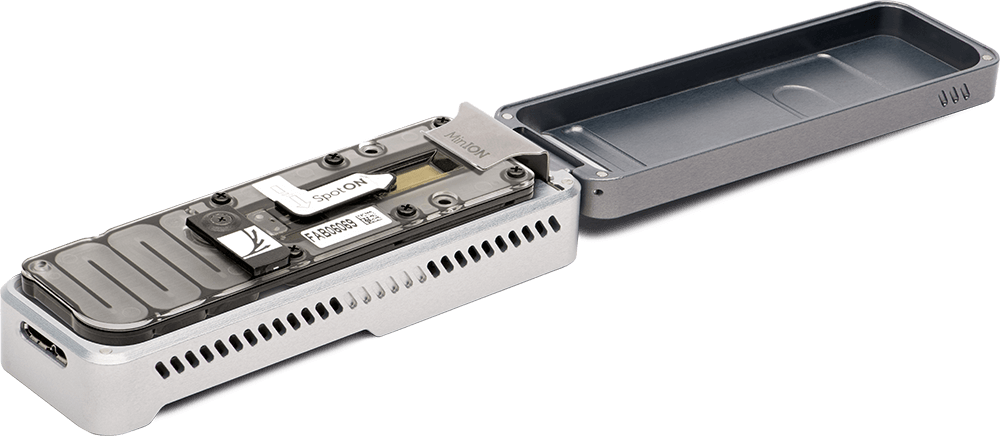
\includegraphics[width=0.5\textwidth]{images/minion}
  \caption{MinION device.}
  \label{fig:minion}
\end{figure}

A nanopore is a hole so small, that only single DNA strand fits in. MinION
uses a protein nanopore set in an electrically resistant polymer membrane. 
An ionic current is passed through the nanopore by setting a voltage across this membrane. If an analyte passes through the pore or near its aperture, 
this event creates a characteristic disruption in the current. Measurement of that current makes it possible to identify the molecule in question \cite{oxford}.

\subsection{Processing of MinION data}
\label{standard}
Raw data produced by MinION device consist of current measures in picoamperes.
Each measured value corresponds to five or six bases passing nanopore called 5-mers or 6-mers (Fig. \ref{fig:kmers}).
Each k-mer is measured several times as passing through a nanopore.

\begin{figure}
  \centering
  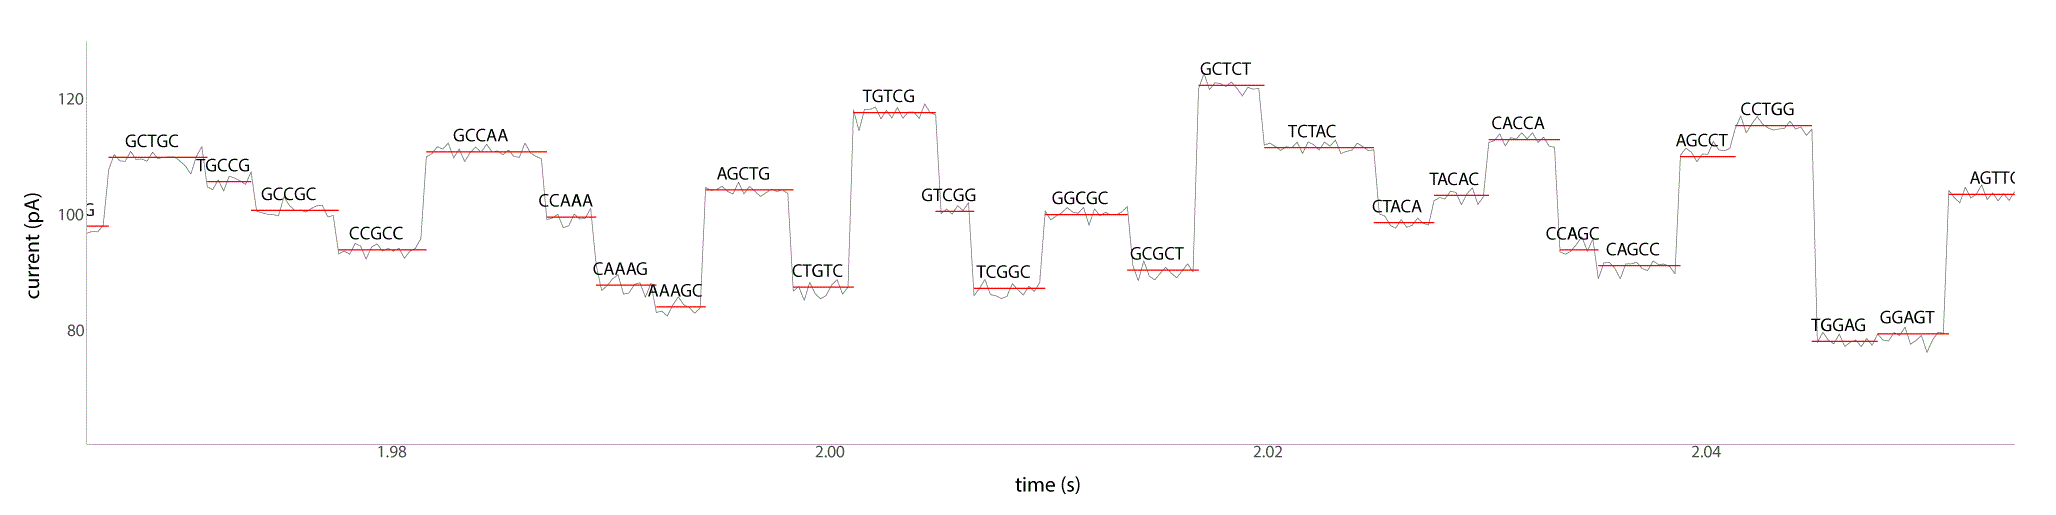
\includegraphics[width=1.0\textwidth]{images/kmers}
  \caption{Raw signal generated by MinION device with corresponding 5-mers \cite{kmersimage}.}
  \label{fig:kmers}
\end{figure}

The MinION device typically produces many reads covering different parts of processed DNA molecule.
The process of translating current measures into a sequence of bases (letters A, C, G, T) is called basecalling. 
It is slow process usually based on hidden Markov model or recurrent neural networks. 

Regular approach to analyzing MinION data is to basecall all reads and find their order and overlap by standard 
sequence aligning algorithms.